%#! platex thesis.tex

%======================================================================
\chapter{Ratio手法によるデータ拡張及び実装}
\label{cha:propose}
本章では,オンライン文字認識用のデータ拡張の新手法としてRatio手法を提案し,実装方法について説明する.
%----------------------------------------------------------------------
\section{Ratio手法}
\label{ratio}
ここでは,オンライン文字におけるデータ拡張の新手法として,文字の縦横比を変更するRatio手法を提案する.先行研究\cite{takahashi}のSRP手法において回転の大きさ,平行移動の大きさは筆者が文字の形を崩さないと判断できる範囲で設定している.そのためデータを100倍に拡張した場合,同じようなデータが増えてしまい学習精度が低くなる原因になる.Ratio手法では文字の縦横比変更を行うので文字のストロークが重なることがなく,文字の形が大きく崩れてしまうことがない.そのため文字の形を崩さない最大のパラメーターでSRP手法を適用した後でも,Ratio手法を用いてさらに拡張できる.またRatio手法は事前に変更比率を定める手法であり,Ratio手法を用いて拡張されたデータはそれぞれが必ず一定の割合で変化しており,少ない倍率でもRatio手法を組み合わせることによってデータが多様化する.SRP手法とRatio手法を組み合わせることによりSRP手法のみで拡張をする場合に比べ,よりデータの多様化を実現することができる.

\textbf{図~\ref{yratio}(a)}に文字の縦横比変更の原理を示す.文字の縦横比変更は$x$座標を基準に行う場合と$y$座標を基準に行う場合がある.
ここでは$y$座標を基準に行う場合を具体的に説明する.1つの単語におけるすべての点のy座標の平均値を取り,すべての点のy座標に対し平均値との大小関係の比較をする.比較結果に応じて,点の移動を行う.文字の拡張比率を$r$,1つの単語上におけるすべての点の$y$座標平均を$\bar{y}$とし,同単語上の任意の点の座標を$(x, y)$としたとき,その点の$y$座標が$\bar{y}$より大きい場合,$y$座標に$y$座標の値の$r$倍を加算し,$\bar{y}$との距離が大きくなる方向に移動させた後の座標$(X, Y)$は 式~\ref{eq:yratio>}で表される.

\begin{equation}
  (X, Y) = (x, y(1+r))
  \label{eq:yratio>}
\end{equation}

一方,$y$座標が$\bar{y}$より小さい場合,$y$座標から$y$座標の値の$r$倍を減算し,$\bar{y}$との距離が大きくなる方向に移動させた後の座標$(X, Y)$は 式~\ref{eq:yratio<}で表される

\begin{equation}
  (X, Y) = (x, y(1-r))
  \label{eq:yratio<}
\end{equation}

この式を単語上のすべての点に用いることで,単語全体の点を単語の$y$座標の平均を基準に移動させ,単語全体を$y$方向に引き伸ばす.
$x$座標を基準に拡張する場合は,これらの式の$x$と$y$を逆にして計算を行う.


\textbf{図~\ref{yratio}(b)}に縦横比率変更前の単語データの例,\textbf{図~\ref{yratio}(c)}に文字の縦横比率を$y$座標を基準に変更後の単語データの例を示す.この処理を,拡張回数ごとに拡張比率$r$と,単語の$x,y$どちらを基準に適応するか変えながら行うことで元のデータとは異なる形の文字・単語を生成する.それを1つの単語データに対して$N$回行い,データ量を$N$倍に拡張する.

$x$座標・$y$座標どちらを基準に比率変更を行うかは$x:y$を$1:2$の割合でランダムに決定している.1つの単語において文字が横方向に並んでいる場合には,全体を$y$座標を基準に縦方向に比率変更を行うのが効果的である.一方単語が1箇所に固まっている場合や斜め方向に書かれている場合には,全体を$x$座標を基準に横方向に比率変更を行うのも効果的であると考えられる.本研究において収集したデータは英語とバングラ語を含んでおり,さらに一般的な文字より雑な文字を扱うため文字の配置が横方向のものだけでなく,斜めや1箇所に集中したものを含んでいる.このため$x:y$を$1:2$の割合とすることでより効果的にデータを多様化させている.

\begin{figure}[tb]
 \centering
  \begin{tabular}{c}
   \begin{minipage}[b]{0.7\hsize}
    \centering
    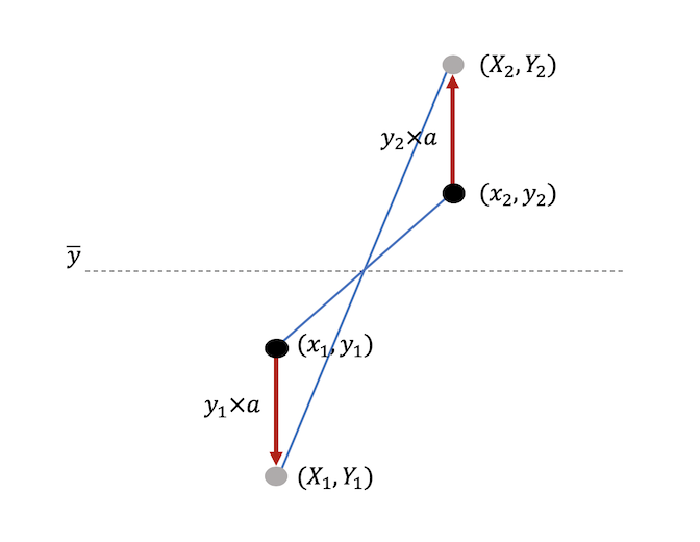
\includegraphics[keepaspectratio,scale=0.7]{img/yratio.eps}\\
    (a)縦横比率変更の原理
   \end{minipage}\\
    \hfill
   \begin{minipage}[b]{0.5\hsize}
    \centering
    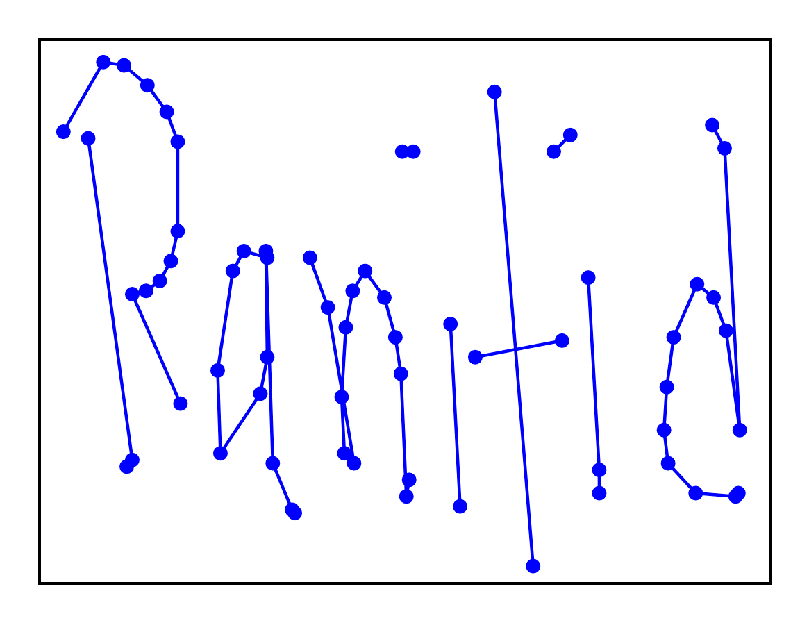
\includegraphics[keepaspectratio,scale=0.5]{img/ranitidCloseBlue.eps}\\
    (b)データ前処理後
   \end{minipage}
   \begin{minipage}[b]{0.5\hsize}
    \centering
    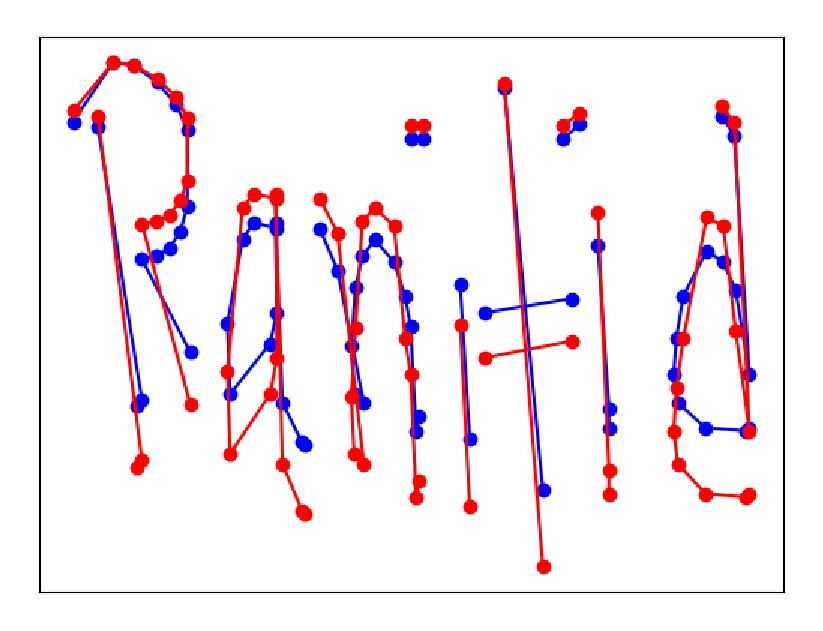
\includegraphics[keepaspectratio,scale=0.5]{img/ranitidRatioRedBlue.eps}\\
    (c)縦横比率変更前(青)と変更後(赤)
   \end{minipage}
  \end{tabular}
 \caption{文字の縦横比率変更}
 \label{yratio}
\end{figure}

\section{実装}
\label{cha:imple}
本章では先行研究で収集したデータについて説明し,本論文でのオンライン手書き医療用語認識手法の実装について説明する.
%----------------------------------------------------------------------
\subsection{データ収集}
\label{sec:collection}
学習に使用したいデータがオープンソースで存在していないため,先行研究\cite{takahashi}において独自に収集しているデータを用いる.本研究では,過去の処方箋データから医療用語コーパスを作成している.コーパスとは,言語を分析するための基礎資料として書き言葉や話し言葉の資料を収集し,研究用の情報を付与したものである.本研究及び先行研究では医療用語の手書き認識を行う.そこで \ref{sec:background}節で述べたPHCの過去の処方箋データからコーパスを作成し,それを機械学習の正解データとして用いている.8324名分の過去の処方箋データは,それぞれの欄が症状,薬名などに分けられる.先行研究では薬名欄に頻出する単語(360語,英語)と医者からのアドバイス欄に頻出する単語(120語,バングラ語)を用いてコーパスを作成し,データ収集を行っている.データ提供者により手書きされた文字は正解データとともにデータベースに保存される.
%
%----------------------------------------------------------------------

\subsection{使用機器・学習モデル構造}
\textbf{図~\ref{equipments}}に使用機器,\textbf{~\tablename~\ref{tab:spec}}に実装環境を示す.機械学習には NVIDIA社の GeForce 1080 が1枚搭載された デスクトップ PC を用いた.\textbf{図~\ref{layers}}に本研究で用いた学習モデルの構造を示す.本研究で用いるデータはデータ長が一定ではないため,データの後ろを$0$でパディングすることでデータ長最大の値である$260$に揃え,学習の入力とした.LSTM層の出力次元数は$300$に設定し,プールサイズの値の平均値をそれぞれ出力するプーリング層を配置した.その後パラメータの数を増やすために全結合層を配置した.なお,過学習を防ぐためプーリング層と全結合層の間にドロップアウト\cite{dropout}をそれぞれ$0.3$の割合で設定した.

\begin{figure}[tb]
 \begin{center}
  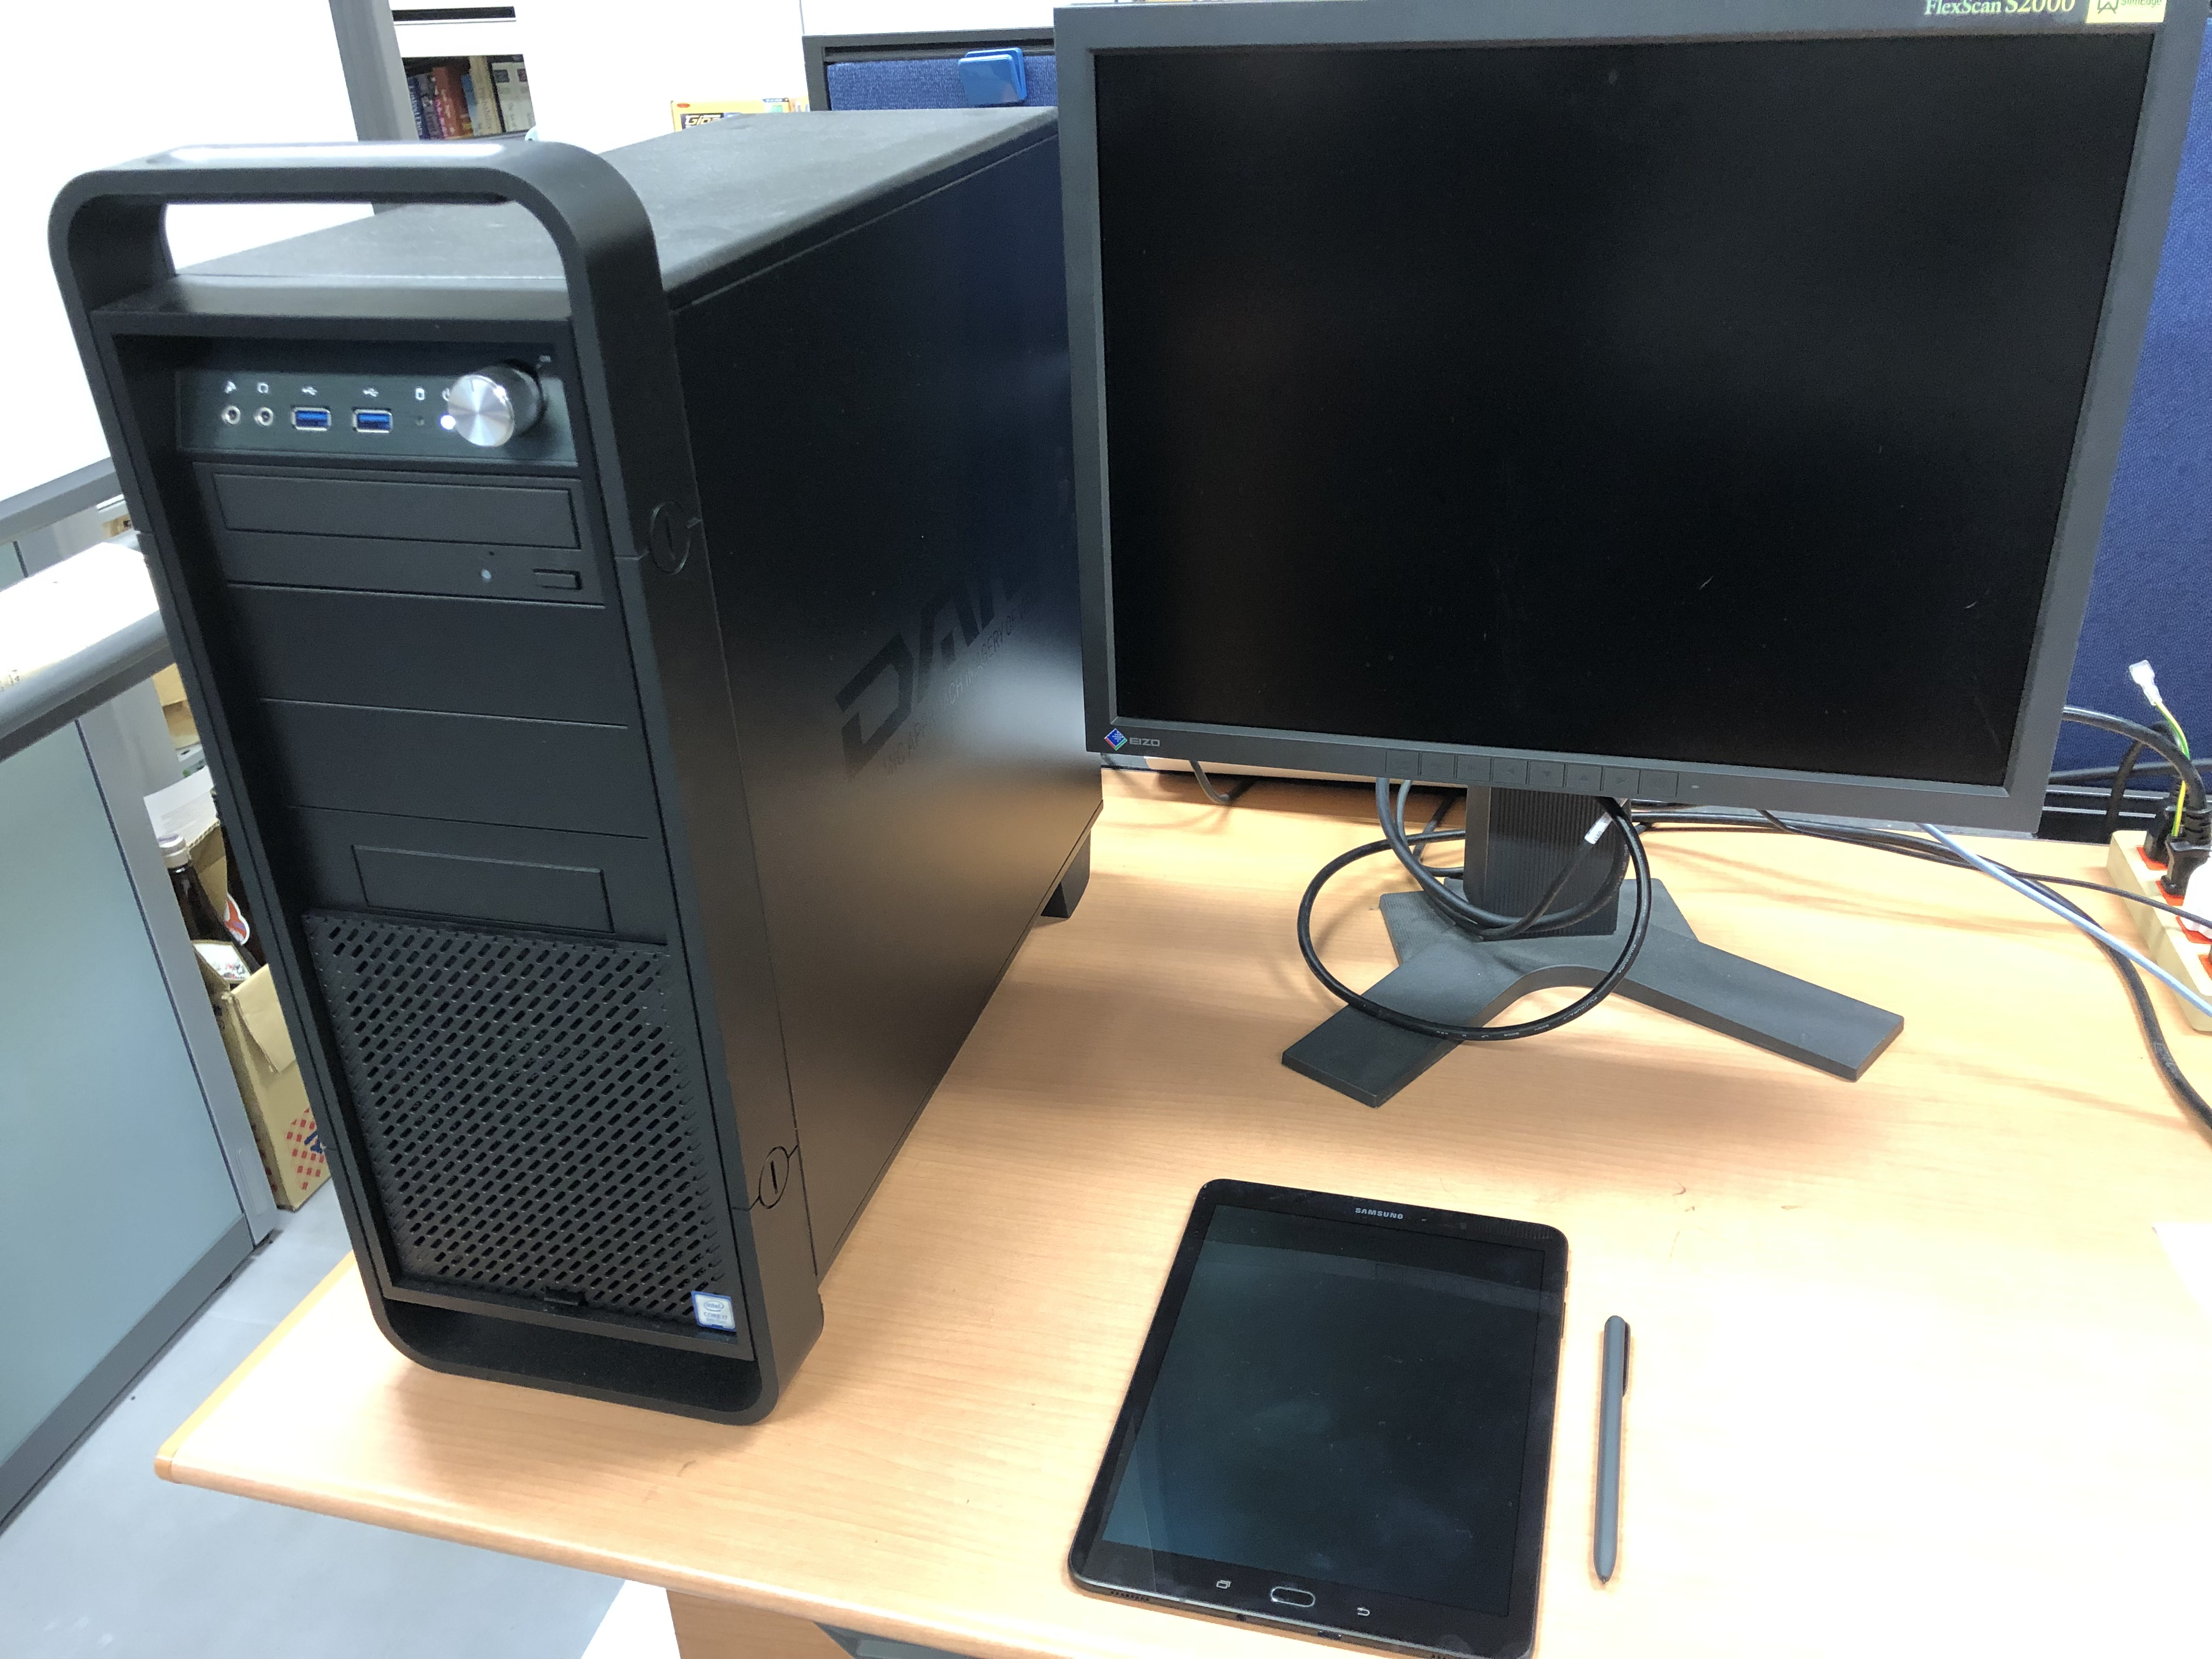
\includegraphics[keepaspectratio, scale=0.1]{img/equipments.png}
  \caption{使用機器}
  \label{equipments}
\end{center}
\end{figure}

\begin{table}[bt]
 \centering
 \caption{実装環境}
 \label{tab:spec}
 \begin{tabular}{ll}\Hline
  OS & \texttt{Ubuntu 16.04}\\
  GPU & \texttt{NVIDIA GeForce 1080}\\
  メモリ & \texttt{8GB}\\
  プロセッサ & \texttt{3.70GHz Intel Core i7-8000K}\\
 \Hline
 \end{tabular}
\end{table}

\begin{figure}[tb]
 \centering
  \begin{tabular}{c}
    \begin{minipage}[b]{0.7\hsize}
     \centering
     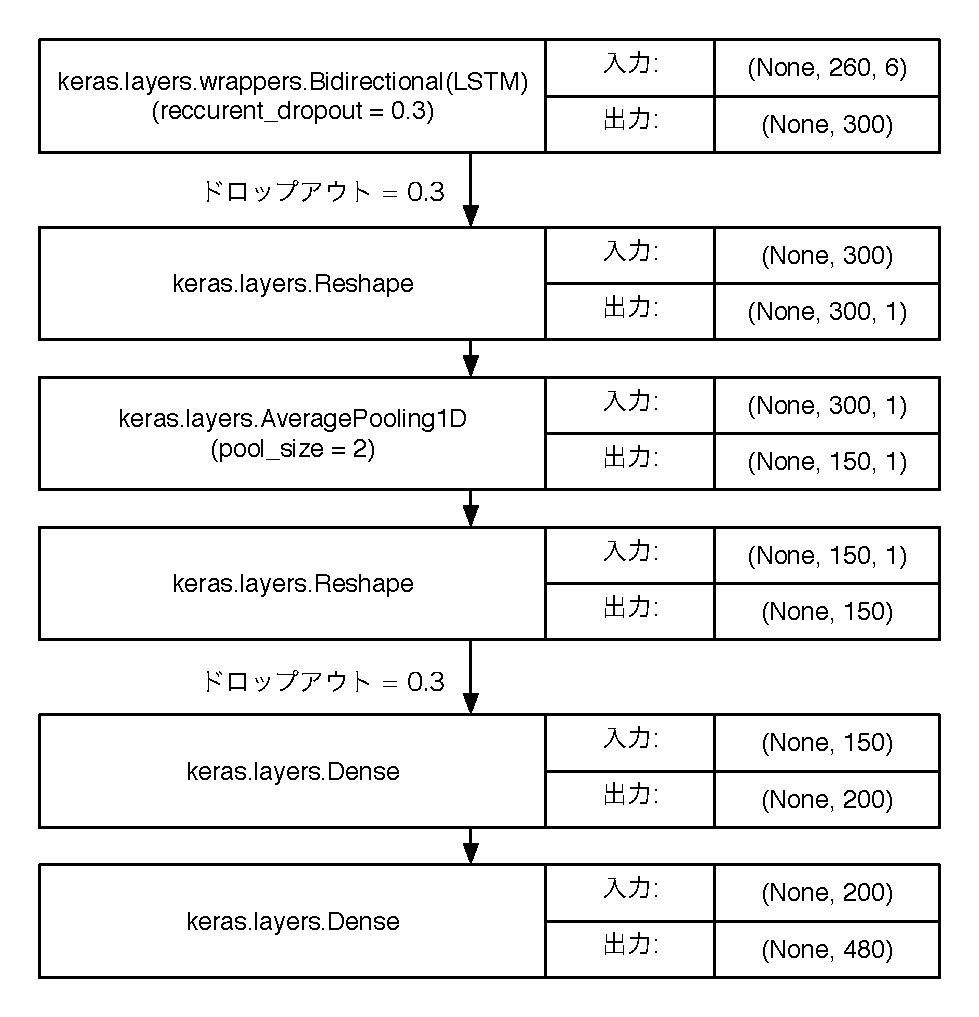
\includegraphics[keepaspectratio,scale=0.7]{img/layers.eps}\\
    \end{minipage}
  \end{tabular}
 \caption{層の構成}
 \label{layers}
\end{figure}



% 以下はRefTeX用
%%% Local Variables:
%%% mode: yatex
%%% TeX-master: "thesis"
%%% End:
